% Template GRASS newsletter - Article
% Language: Latex
%

% Head

\title{Evapotranspiration mapping with Landsat 5TM in GRASS GIS}
\subtitle{Manual}
\author{Pakparvar M. (U. Ghent, Belgium) and GRASS Development Team}

\maketitle
\section{Introduction}

This manual aims at explaining step-by-step how to prepare and process Landsat 5 TM imagery data after downloading it from GLOVIS (http://glovis.usgs.gov) The location of study area is a water harvesting (floodwater spreading) project is being set up in South central Iran (Kowsar research station, Gareh Bygone, fars Province). Time series of Et maps is needed for integration and calculation the hydrologic balance. The WRS-2 path=164 and row=040. The site is located south-central East border of the image. Fig.~\ref{fig:gipe000}\newline

%\setkeys{Gin}{width=1\textwidth}
\begin{figure}[htbp]
   \centering
   %name of your graphic, without the path AND in PNG (screnshots etc)/PDF (drawings) format:
   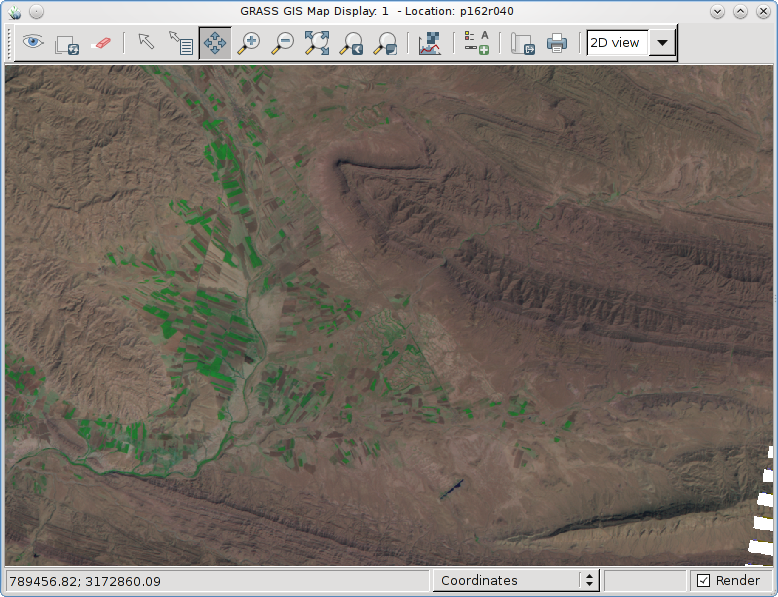
\includegraphics[scale=0.4]{gipe000.png}
   %caption of the figure
   \caption{Study Area in p162r040 of Landsat 5TM}
   %label of the figure, which has to correspond to \ref{}:
   \label{fig:gipe000}
\end{figure}

\section{Downloading the image}
Scenes from the Landsat archive are available at no charge, processed to Standard Terrain Correction (Level 1T). While some scenes do not have the ground-control or elevation data necessary to perform L1T correction, the best level of correction is applied. More details at \href{http://landsat.usgs.gov/products_productinformation.php}{Landsat Product Information}.\newline

The \href{http://glovis.usgs.gov/BrowseBrowser.shtml}{USGS Global Visualization Viewer} is a quick and easy online search and order tool for selected satellite and aerial data. When the USGS Global Visualization Viewer is open, the Global View is seen.\newline

There is option to add the known latitude and longitude or select the desired region by cursor tool.\newline

A new windows is appeared to search and request the imagery. This stage needs to install the last version of Java program and needs to permit the pop up to run by the windows firewall.
In new window go to Collection > Landsat Archive > to have access to updated landsat images or Collection > Landsat Legacy Collections for old images.\newline

After klicking on desired  category of  images it is possible to see the scenes on the screen. There are options in bottom left to determine the year and month of interest or pushing on "nest scene" , "previous scene". In case of availability of desired scene for downloading, a red alarm is appeared top of screen mentioning "Downloadable".  Klick on Add button to add the image in request list.\newline

In case of the image to be downloadable push the Download button otherwise the Submit button.\newline  

%\setkeys{Gin}{width=1\textwidth}
\begin{figure}[htbp]
   \centering
   %name of your graphic, without the path AND in PNG (screnshots etc)/PDF (drawings) format:
   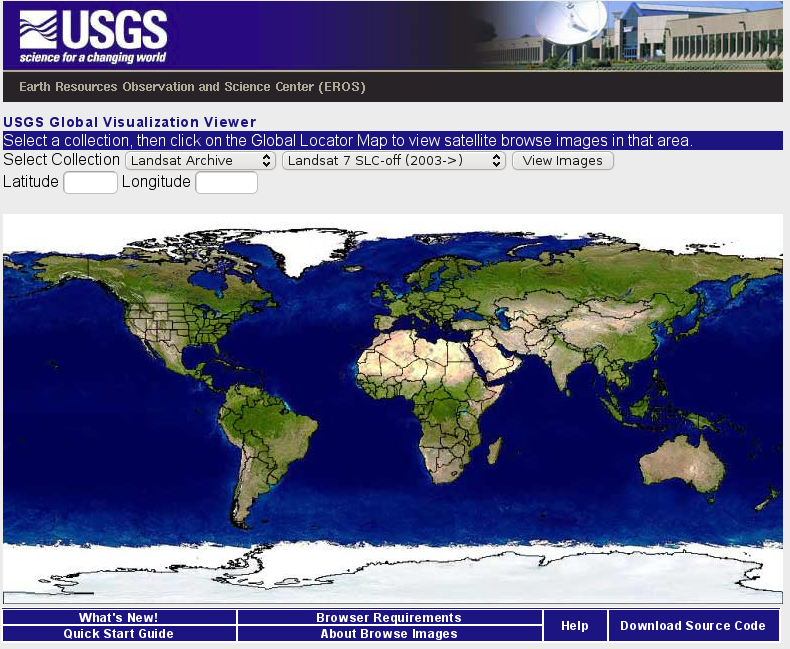
\includegraphics[scale=0.4]{gipe001.png}
   %caption of the figure
   \caption{Glovis Main Page}
   %label of the figure, which has to correspond to \ref{}:
   \label{fig:gipe001}
\end{figure}

%\setkeys{Gin}{width=1\textwidth}
\begin{figure}[htbp]
   \centering
   %name of your graphic, without the path AND in PNG (screnshots etc)/PDF (drawings) format:
   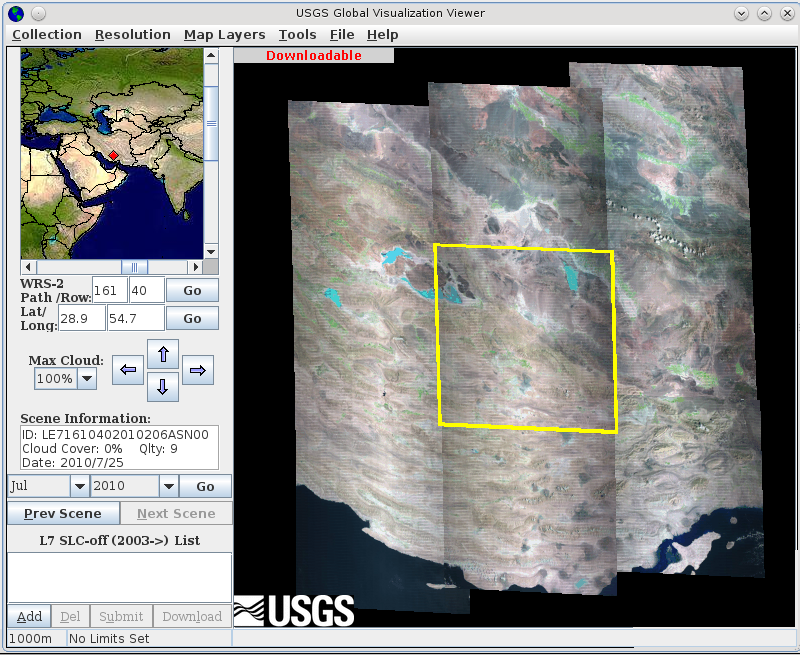
\includegraphics[scale=0.35]{gipe002.png}
   %caption of the figure
   \caption{Search within Glovis}
   %label of the figure, which has to correspond to \ref{}:
   \label{fig:gipe002}
\end{figure}

For submitting the request it is needed to register to the USGS site. After a while a massage will be sent to the email of subscriber giving a link to give access for downloading the image.\newline

There is an easier way to request the images of successive time series. The USGS website has prepared a new envaironment of searching tool for the image requaest is called earth explorer. The link \href{http://edcsns17.cr.usgs.gov/NewEarthExplorer}{NewEarthExplorer} gives the access to the search window that looks like the google earth. There are 4 label at the top to determine the the images. In Search criteria, start and end date of the time series, exact lat. Long. and/or name of the location can be determined. In Data set it is possible to select the type of image. In Additional criteria there are options to  start and end path and row of the interest and some other criteria. In Result label, all of the scenes of interest will be shown, downloaded or requested. Subscription to the Earth Explorer is also needed for the request. There is  a limitation of 100 scenes per subscriber.\newline

%\setkeys{Gin}{width=1\textwidth}
\begin{figure}[htbp]
   \centering
   %name of your graphic, without the path AND in PNG (screnshots etc)/PDF (drawings) format:
   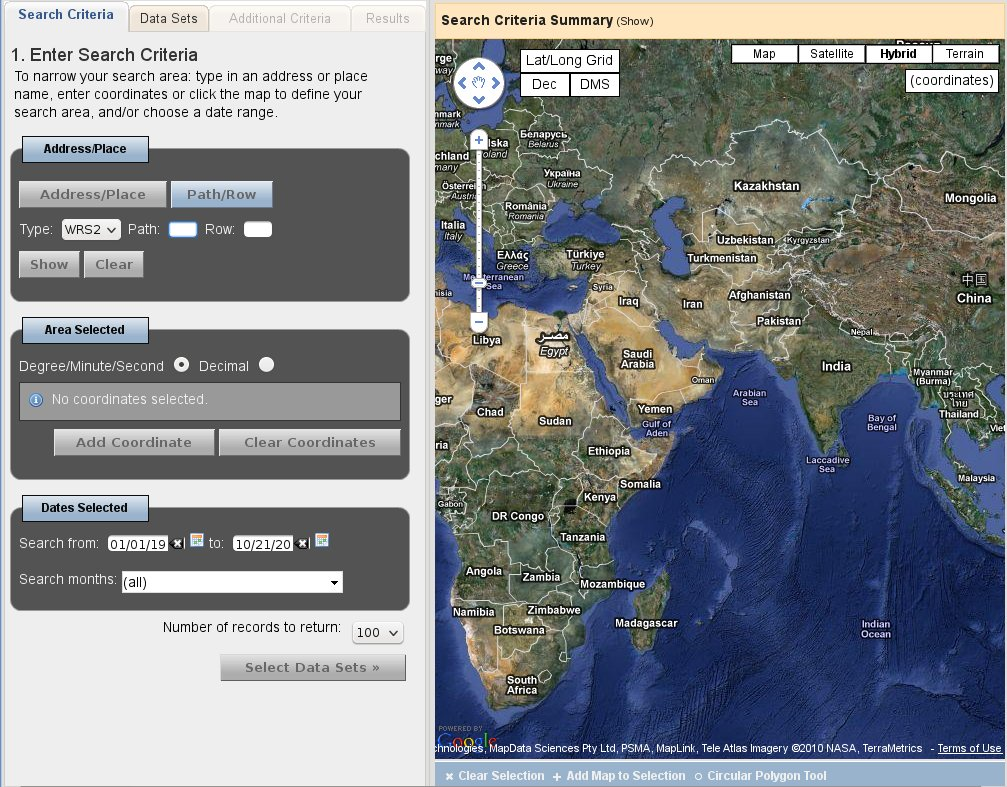
\includegraphics[scale=0.3]{gipe003.png}
   %caption of the figure
   \caption{Search Criteria within Glovis}
   %label of the figure, which has to correspond to \ref{}:
   \label{fig:gipe003}
\end{figure}

In case of downloadable, a green downward arrow is appeared on the resulted sample image otherwise the sign of add to shop (like the shopping cart) is seen and has to be pushed changing it to green color.\newline

%\setkeys{Gin}{width=1\textwidth}
\begin{figure}[htbp]
   \centering
   %name of your graphic, without the path AND in PNG (screnshots etc)/PDF (drawings) format:
   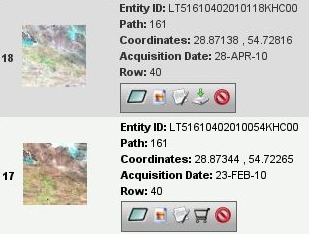
\includegraphics[scale=0.5]{gipe004.png}
   %caption of the figure	
   \caption{Shopping Cart Items}
   %label of the figure, which has to correspond to \ref{}:
   \label{fig:gipe004}
\end{figure}

In case of submit and request a new menu is shown and needs a name for this request and some other criteria such as start and end time for the request. This timing is duration of the request and not the acquisition  time of the images. \newline

%\setkeys{Gin}{width=1\textwidth}
\begin{figure}[htbp]
   \centering
   %name of your graphic, without the path AND in PNG (screnshots etc)/PDF (drawings) format:
   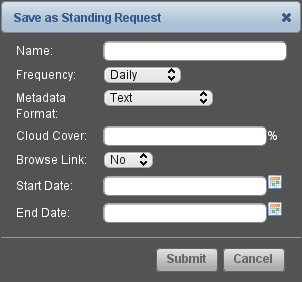
\includegraphics[scale=0.4]{gipe005.png}
   %caption of the figure
   \caption{Save as Standing Request}
   %label of the figure, which has to correspond to \ref{}:
   \label{fig:gipe005}
\end{figure}

Afterward a message will be sent to the subscriber email to give access to downloading the images.\newline

All of the images are in the Zip format and should be collected in a unique folder.\newline

While most Landsat scenes are processed as Level 1T (precision and terrain corrected), certain scenes do not have ground-control or elevation data necessary for precision or terrain correction. In these cases the best level of correction is applied (Level 1G-systematic or Level 1Gt-systematic terrain). Additionally, the majority of all archived Landsat 1-5 MSS scenes, as well as a select number of Landsat 4-5 TM scenes are processed only as Level 1G (systematic) due to processing constraints. However, improvements to production capabilities are being investigated, which will allow more scenes to be processed at a higher level with a shorter processing time. The processing level of a downloaded scene is found in the metadata (MTL.txt) or processing history (WO.txt) files which are delivered with the data band files and other ancillary data.\newline

More details can be found at \href{http://landsat.usgs.gov/products\_productinformation.php}{landsat.usgs.gov} \newline


\section{Implementation environment}
GRASS GIS (Geographic resources Analysis Support System) is an open source, Free GIS software that operates on various platforms. Therefore binaries can be downloaded and installed on Unix, Linux, MS-Windows or MAC OS X workstation.\newline

The currently last version GRASS 7.0 is downloadable at www.grass.osgeo.org. It has a windows version in which the windows users can easily work in its environment.\newline

The new modules are all incorporated in the GRASS Image Processing Environment (GIPE) folder. The modules are accessible from the \href{http://trac.osgeo.org/grass/browser/grass-addons/gipe}{trac.osgeo.org} website.\newline

After downloading and installing the software, an specific work area should be determined for first time of opening. All of the files imported and newly generated in GRASS are located in the determined path such as "C:/GRASSDATA/Landsat5/PERMANENT". \newline

Naming of the folders is optional except for the "PERMANENT" that is GRASS default name for administrator specific working environment that is called MAPSET. Every user has a username and password and have access to their own folders which is determined by admin. \newline

Image container folder is not the same as working folder. GRASS generated files are in the binary format and can not easily read by normal windows programs. Therefore, Copy and pasting as well as the exporting of these files must perform inside the GRASS. \newline

Linux users have easier and simpler access to script writing for automation of a repeatable task for faster and (man-made) error free results. But it doesn't mean the Windows users can not use it properly.\newline

Starting the GRASS in Windows is performed by klicking on the exe file. In Linux it should be written "grass70" (70 means version 7.0) in Terminal area and push the enter key.\newline
 
After the first time opening of the GRASS, the following menu is appeared to select the working area. There are possibilities to make a new location for the project and new name for mapset. Renaming the older mapsets can only be done in this menu and must not perform in the other programs (such as windows explorer). Followings are some examples of naming:\newline

Main working folder for GRASS data: GRASSDATA;\newline
Name of the specific project: L5;\newline
Name of the mapset: PERMANENT.\newline

%\setkeys{Gin}{width=1\textwidth}
\begin{figure}[htbp]
   \centering
   %name of your graphic, without the path AND in PNG (screnshots etc)/PDF (drawings) format:
   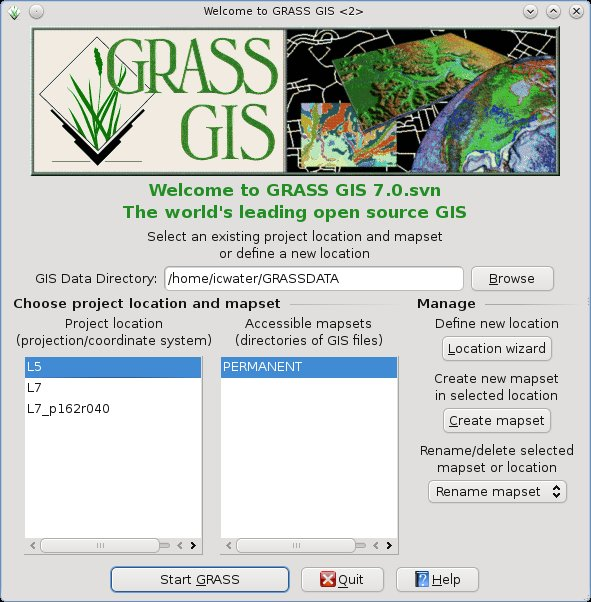
\includegraphics[scale=0.4]{gipe006.png}
   %caption of the figure
   \caption{GRASS GIS Welcome Interface}
   %label of the figure, which has to correspond to \ref{}:
   \label{fig:gipe006}
\end{figure}

Starting the GRASS shows three new windows:\newline
GRASS Layer management: for main data analysis;\newline
GRASS Map Display for viewing the resulted layers;\newline
CLI (Command Line Interface): for scripting.\newline

%\setkeys{Gin}{width=1\textwidth}
\begin{figure}[htbp]
   \centering
   %name of your graphic, without the path AND in PNG (screnshots etc)/PDF (drawings) format:
   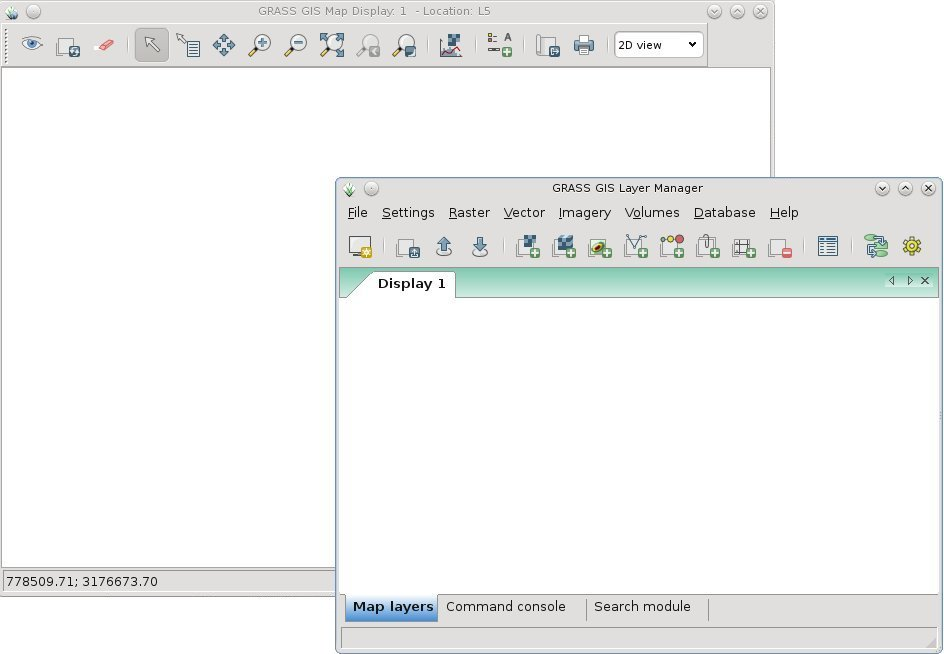
\includegraphics[scale=0.3]{gipe007.png}
   %caption of the figure
   \caption{GRASS GIS Manager and Map Display}
   %label of the figure, which has to correspond to \ref{}:
   \label{fig:gipe007}
\end{figure}	

After opening the GRASS It is also possible to change the working directory. In GRASS Layer Management go to Settings/GRASS working Environment/Change Location and mapset. Then it is possible change the working area.\newline

%\setkeys{Gin}{width=1\textwidth}
\begin{figure}[htbp]
   \centering
   %name of your graphic, without the path AND in PNG (screnshots etc)/PDF (drawings) format:
   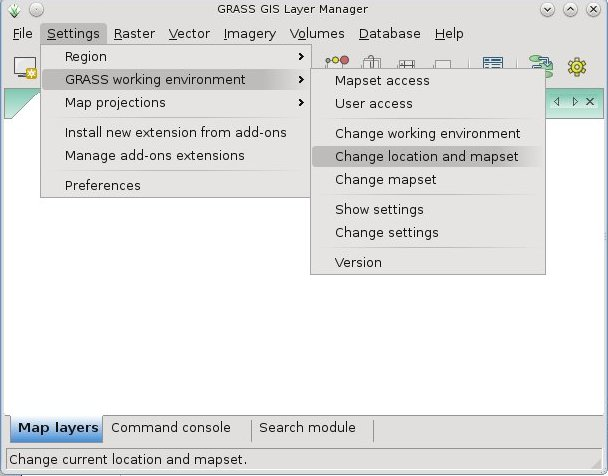
\includegraphics[scale=0.4]{gipe008.png}
   %caption of the figure
   \caption{Change Location and Mapset}
   %label of the figure, which has to correspond to \ref{}:
   \label{fig:gipe008}
\end{figure}	

Scripting in GRASS helps the user to do the tasks fast. Scripts are in the format of C programing language. For writing and executing a script, first the location should be checked (where we are in hard disk?). To do this:\newline
Type pwd and press Enter\newline
\begin{smallverbatim}
>pwd
>/home/GRASSDATA/L5
\end{smallverbatim}

"pwd" means Path to Working Directory and will show the path that you are in now.\newline
For changing to desired path\newline
Type cd and space Folder/Sub folder and Enter\newline 
\begin{smallverbatim}
>cd home/RSDATA/Landsat5
>/home/RSDATA/Landsaat5
\end{smallverbatim}

Scripts now work in the correct directory.\newline 

\section{Preparation and import in GRASS GIS}
GLOVIS is giving access to download a Landsat 5TM dataset in the form of a tarball (.tar.gz), which is a compressed format. This format compresses the files much more than the normal zip format. Decompressing the tarball for each available image in the directory can be done by the common Windows unzipping softwares one by one.\newline\linebreak
In Linux it is possible to decompress the files by using the script mentioned in \ref{appendixA}-1.\newline
Once this is done, start GRASS GIS and create a new location from the New Location wizard, name it as the Path and Row of the images (i.e. p162r040), and use any of the landsat5.TIF images available as a reference image to get the projection system and other information from.\newline
There is a need to import and rename the images inside the GRASS with the extensions in number format because the preprocessing module "i.landsat.toar" which imports DN and convert them into either radiance or reflectance is using a base name with numbered extensions.  For instance:\newline\linebreak
Landsat 5 TM:\newline
L5162040\_04020090705\_B10.TIF \newline
=> L5162040\_04020090705.1\newline
The same for the other bands till band 7.0\newline
L5162040\_04020090705\_B70.TIF \newline
=> L5162040\_04020090705.7\newline\linebreak
Landsat 7 ETM+:\newline
L71161040\_04020100607\_B10.TIF \newline
=> L7\_161040\_04020100607.1\newline
The same for the other bands till band 7.0 except for the bands 6.1 and 6.2\newline
L71161040\_04020100607\_B61.TIF \newline
=> L7\_161040\_04020100607.61\newline
L72161040\_04020100607\_B62.TIF \newline
=> L7\_161040\_04020100607.62\newline\linebreak
It is possible to do one by one in GRASS Import menu. For every band that is selected from the image container folder, an output file should be written as the new file naming system mentioned above.\newline

%\setkeys{Gin}{width=1\textwidth}
\begin{figure}[htbp]
   \centering
   %name of your graphic, without the path AND in PNG (screnshots etc)/PDF (drawings) format:
   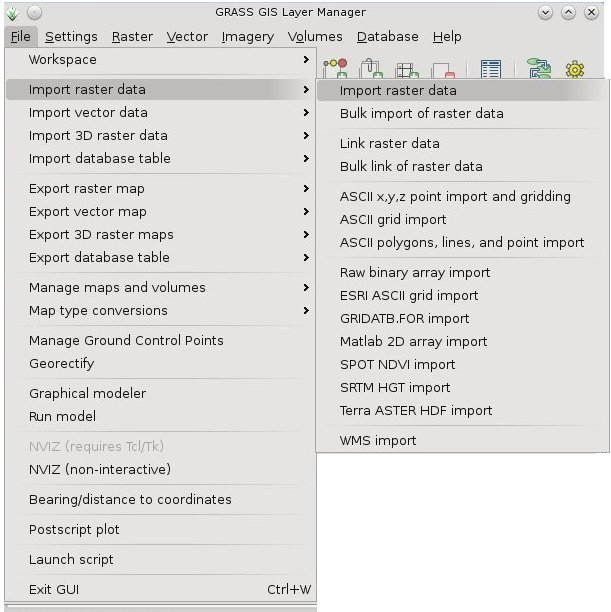
\includegraphics[scale=0.4]{gipe009.png}
   %caption of the figure
   \caption{Accessing Raster Import}
   %label of the figure, which has to correspond to \ref{}:
   \label{fig:gipe009}
\end{figure}

%\setkeys{Gin}{width=1\textwidth}
\begin{figure}[htbp]
   \centering
   %name of your graphic, without the path AND in PNG (screnshots etc)/PDF (drawings) format:
   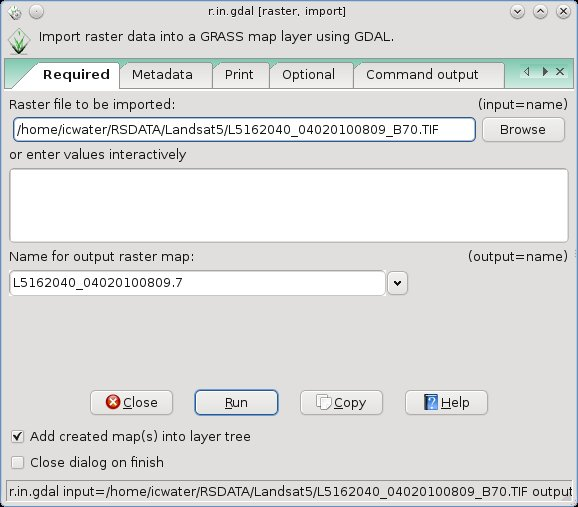
\includegraphics[scale=0.4]{gipe010.png}
   %caption of the figure
   \caption{Raster Import Module}
   %label of the figure, which has to correspond to \ref{}:
   \label{fig:gipe010}
\end{figure}

It is possible also to import and rename the images by using the command line. Once inside the p162r040 location, access the Command Line Interface (CLI) and "cd" to the directory where all of your newly decompressed images are located. In that directory, launch the script mentioned in \ref{appendixA}-2.\newline

Imported images are now in the working environment of the GRASS (i.e. /home/GRASSDATA/L5/PERMANENT). So, it is impossible for common programs to access to and open the imported images except after the exporting.\newline

\section{Preprocessing}
\subsection{Determination of the region}
In GRASS it is possible to set the region of interest as a pre determined part of the image(s) whereby all of the processes will be done based on the data of  this region. Unlike the other softwares, it doesn't mean a separate sub image file to be produced. This activity reduces the time and increases the speed of processing  intensely.\newline

In GRASS Layer Manager push on the "Add various raster" button and select Add RGB Mapp Layer. In new window select desired band for every Red, Green or Blue band and press OK.\newline

%\setkeys{Gin}{width=1\textwidth}
\begin{figure}[htbp]
   \centering
   %name of your graphic, without the path AND in PNG (screnshots etc)/PDF (drawings) format:
   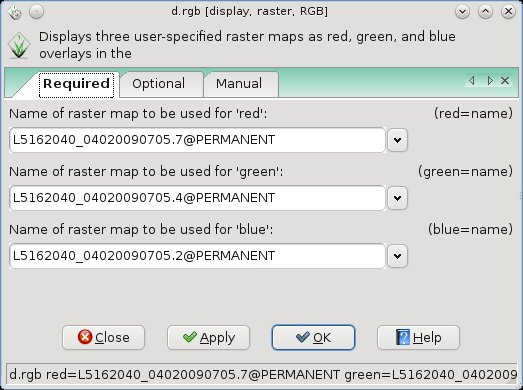
\includegraphics[scale=0.4]{gipe011.png}
   %caption of the figure
   \caption{Raster RGB Display}
   %label of the figure, which has to correspond to \ref{}:
   \label{fig:gipe011}
\end{figure}

The selected composition (is called false color composite) is shown In GRASS Map Display. Once in this window zoom to interested area by zoom tool. To determine this region as the interested part of images to be processed, push the icone "zoom options" and select set the computational region from the map. It is possible also to save specifications of the region from the map.
Selected region in Map display will be the only part of image that attends to the further processes.\newline

\subsection{Georeferencing} 
According to the GLOVIS, as mentioned before, most Landsat scenes are processed as Level 1T (precision and terrain corrected), certain scenes do not have ground-control or elevation data necessary for precision or terrain correction. In these cases the best level of correction is applied (Level 1G-systematic or Level 1Gt-systematic terrain). So there is no need to perform geometric correction for newly downloaded landsat 5 TM or landsat 7 ETM images.\newline

In case of need, it is possible to do georeferencing in the GRASS that is called rectification.  This module rectifies an image by computing a coordinate transformation for each pixel in the image based on the control points. The procedure and steps is mentioned in detail in: "r.rectify" manual that is accessible in Grass Layer Management/Imagery/Rectify Image or Raster.\newline

\subsection{Change DN to radiance and reflectance at top of atmosphere}
Radiance and reflectance are the major basic input layer in ET calculation. DN can be converted to radiance by using the Lmax and Lmin of the spectral bands that is mentioned in the met or mtl files.\newline

Lmax and Lmin are the extreme values of actual radiance is sensed by the satellite sensor for each band. QCALmax and QCALmin are the extreme values of the DNs in each band and commonly is between 0-255 or 1 -255. The radiance value for each pixel is calculated by Gain and Bios data.\newline

\begin{smallverbatim}
Gain = (Lmax - Lmin) / (QCALmax - QCALmin) 
Bias = Lmin - gain * QCALmin 
Radiance = gain * DN + bias 
\end{smallverbatim}

The top of atmosphere reflectance (toar) is calculated by dividing the actual radiance at sensor with the potential radiance (sun incoming irradiance) at the top of atmosphere, which is calculated by using the sun elevation and astronomical equations.\newline
Then, to calculate at-sensor reflectance the equations are: \newline
\begin{smallverbatim}
sun_radiance = [Esun * sin(e)] / (PI * d^2) 
reflectance = radiance / sun_radiance 
\end{smallverbatim}

where, d is the earth-sun distance in astronomical units, e is the solar elevation angle, and Esun is the mean solar exo-atmospheric irradiance in W/(m2 * µm). \newline
Once the images are all imported in GRASS, go to Imagery/satellite image tools/Landsat DN to radiance-reflectance and run the i.landsat.toar module. \newline

%\setkeys{Gin}{width=1\textwidth}
\begin{figure}[htbp]
   \centering
   %name of your graphic, without the path AND in PNG (screnshots etc)/PDF (drawings) format:
   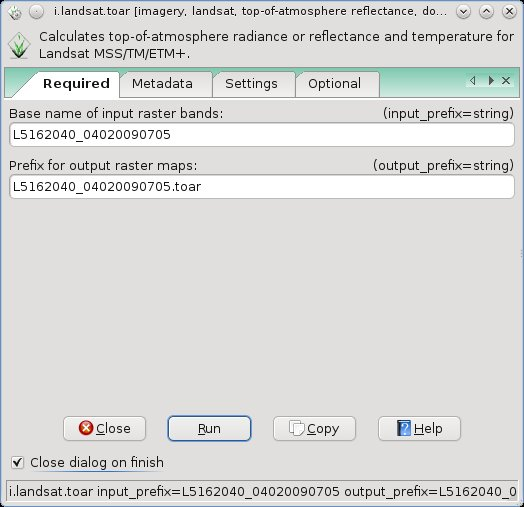
\includegraphics[scale=0.4]{gipe012.png}
   %caption of the figure
   \caption{i.landsat.toar Module}
   %label of the figure, which has to correspond to \ref{}:
   \label{fig:gipe012}
\end{figure}

Fill in the input file name and choose a new name for output file reminding the TOAR conversion has been applied to new file.\newline

The name of input file must not be included of the extension values. Assigning the main part of the image itself let the software.\newline 

By default, all of the necessary input data is read from the "*.met" file that is present in the working directory. If the "*.mtl" is present rather than "*.met", it must be mentioned in Metadata section. Check the square for "Landsat TM5 has a .mtl instead of .met file.\newline

%\setkeys{Gin}{width=1\textwidth}
\begin{figure}[htbp]
   \centering
   %name of your graphic, without the path AND in PNG (screnshots etc)/PDF (drawings) format:
   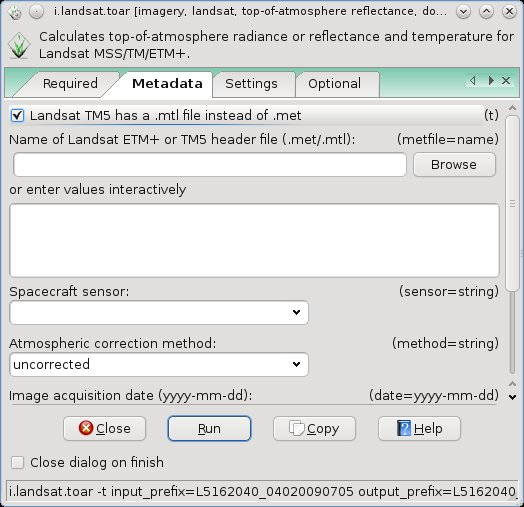
\includegraphics[scale=0.4]{gipe013.png}
   %caption of the figure
   \caption{i.landsat.toar Module, L5TM with MTL}
   %label of the figure, which has to correspond to \ref{}:
   \label{fig:gipe013}
\end{figure}

The output file is the reflectance by default. In the case of need to make the output radiance, it should mention in the Settings section.  Check the square for "output at-sensor radiance for all bands".\newline
Default reflectance output is more favorite because it will speed up the atmospheric correction in next step. But in some other steps there is a need for output radiance. So it is better to produce both radiance and reflectance by twice application of i.landsat.toar with checking and unchecking the  option of the radiance output file. \newline

%\setkeys{Gin}{width=1\textwidth}
\begin{figure}[htbp]
   \centering
   %name of your graphic, without the path AND in PNG (screnshots etc)/PDF (drawings) format:
   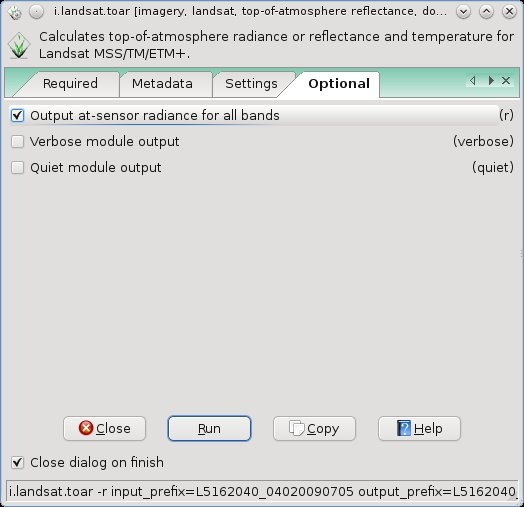
\includegraphics[scale=0.4]{gipe014.png}
   %caption of the figure
   \caption{i.landsat.toar Module, output in Radiance}
   %label of the figure, which has to correspond to \ref{}:
   \label{fig:gipe014}
\end{figure}

\subsection{Atmospheric correction} 
Natural light emitted from the Sun is not polarized. Before it enters the Earth's atmosphere, its intensity remains mostly unchanged and unaffected by the retardation of electric and magnetic components. However after interacting with atmospheric molecules and particles, the unpolarized light may become partially polarized. The degree of polarization depends on the type of scattering event. In the actual case, the signal is perturbed by the atmosphere. Only a fraction of the photons coming from the target reaches the satellite sensor, typically 80\%  at 0.45 μm and 50\% at 0.45  μm, so that the target seems less reflecting. The missing photons have been lost through two processes: absorption and scattering. Atmospheric correction minimizes the errors arise from both two sources.\newline
Through the atmospheric correction, radiance at top of the atmosphere is converted to radiance at the earth surface.\newline
There are two main tools for Atmospheric correction inside the GRASS.\newline

\subsubsection{Dark Object Subtraction (DOS)}
Dark Object Subtraction is one of the simplified methods that is implemented in i.landsat.toar module. It assumes a value called Path-radiance to subtract from all of the pixell's radiance value. \newline

Path-radiance is computed  by subtraction of the Sun\_ radiance from the dark object radiance. So, the equations are:\newline

\begin{smallverbatim}
Surface_radiance = \
 (at-sensor_radiance - radiance_path)

Radiance_path = \
 (dark_radiance - percent* Sun_radiance)   

Sun_radiance = \
 TAUv * [Esun * sin(e) * TAUz + Esky] / (PI * d^2) 
\end{smallverbatim}

Where, percent is a value between 0.0 and 1.0 (usually 0.01), Esky is the diffuse sky irradiance, TAUz is the atmospheric transmittance along the path from the sun to the ground surface, and TAUv is the atmospheric transmittance along the path from the ground surface to the sensor. radiance\_dark is the at-sensor radiance calculated from the darkest object, i.e. DN with a least 'dark\_parameter' (usually 1000) pixels for the entire image. There are four methods of DOS inside the GRASS assuming different values:\newline

\begin{smallverbatim}
DOS1: TAUv = 1.0, TAUz = 1.0 and Esky = 0.0 

DOS2: TAUv = 1.0, Esky = 0.0, \
 and TAUz = sin(e) for all bands with \
 maximum wave length less than 1. \
 (i.e. bands 4-6 MSS, 1-4 TM, and 1-4 ETM+) \
 other bands TAUz = 1.0
 
DOS2b: 

DOS3: TAUv = exp[-t/cos(sat_zenith)], \
 TAUz = exp[-t/sin(e)], Esky = rayleigh
 
DOS4: TAUv = exp[-t/cos(sat_zenith)], \
 TAUz = exp[-t/sin(e)], Esky = PI * radiance_dark  
\end{smallverbatim}

In case of using DOS methods while in i.landsat.toar go to Metadata section and select one of the desired DOS methods of atmospheric correction and the kind of sensor (i.e TM5) and continue  to  convert DN to radiance and reflectance. \newline

In this case, the output file is reflectance or radiance that is atmospherically corrected (by DOS method) and must not be inserted to landsat atmospheric correction module "i.atcorr". \newline

%\setkeys{Gin}{width=1\textwidth}
\begin{figure}[htbp]
   \centering
   %name of your graphic, without the path AND in PNG (screnshots etc)/PDF (drawings) format:
   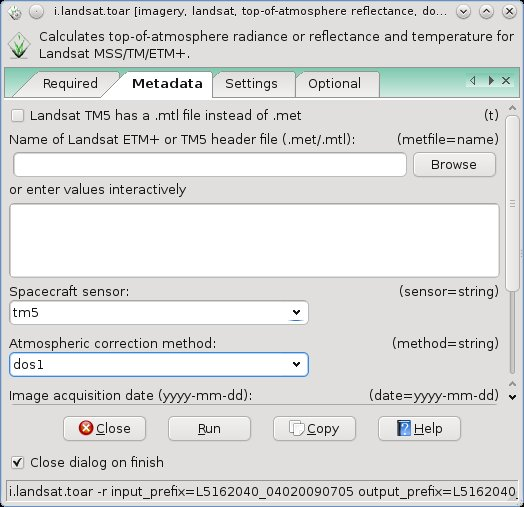
\includegraphics[scale=0.4]{gipe015.png}
   %caption of the figure
   \caption{i.landsat.toar Module, DOS1 model enabled}
   %label of the figure, which has to correspond to \ref{}:
   \label{fig:gipe015}
\end{figure}

The best method of atmospheric correction by the DOS concept can be verified by doing the comparison between the check points of final ET maps (based on each DOS method) with the ground truth data.\newline

\subsubsection{The 6S atmospheric correction model}

The module i.atcorr applies the 6S method to correct the atmospheric errors which is supposed to be the most accurate but input demanding procedure.\newline
6S (Second Simulation of a Satellite Signal in the Solar Spectrum) is an advanced radiative transfer system designed to simulate the reflection of solar radiation by a coupled atmosphere-surface system for a wide range of atmospheric, spectral and geometrical conditions.\newline 
At this point, if a "Dark Object Subtraction" atmospheric correction has not been computed in "i.landsat.toar", then an atmospheric correction must be applied to the TOAR radiance/reflectance values coming from "i.landsat.toar". This is done using "i.atcorr" module. This module is a port of 6S atmospheric correction model.
Atmospheric correction in GRASS can be done in Imageray/Satellite image tools/Atmospheric correction that applies the i.atcorr module.\newline
Parameterization of the i.atcorr is being done inside a text file including the below information (called parameter file).\newline\linebreak 
7                        - geometrical conditions=Landsat 5 TM\newline
7 5 6.30 51.410 24.234   - month day hh.ddd longitude latitude ("hh.ddd" is in decimal hours GMT)\newline
6                        - atmospheric mode=us standard 62\newline
1                        - aerosols model=continental\newline
9                        - visibility [km] (aerosol model concentration), not used as there is raster input\newline
-1.200                   - mean target elevation above sea level [km] (here 1200m asl), not used as there is raster input\newline
-1000                    - sensor height (here, sensor on board a satellite)\newline
30                       - 'i'th band of TM Landsat 5\newline

The figures at the left side are the parameters and the texts in the right side are the defenitions. The text file must be prepared before and browse inside the i.atcorr. The needed information are mentioned in the manual of i.atcorr. Some explanations are as follow.\newline

Line 1 is included of geometric conditions and the correct number can be found in the section A of i.atcorr manual. For landsat 5 tm the number is 7.\newline
Line 2 is mentioning the specifications of the image that is mentioned in mtl file. Latitude and longitudes are the geographic location of the center of region. If the position is not available in longitude-latitude (WGS84), the m.proj conversion module can be used to reproject from a different projection. It also can be accessed in  GRASS/Raster/Develop raster map/Reproject  raster map.\newline
After reprojection the location of the center of the region can be determined by g.region module.\newline
In line 3 the atmospheric model must be entered. The possible models are being mentioned in i.atcorr manual section B. In case of access to the radio sound weather data of the region, it is possible to include the user owned data. In this case it should be mentioned 7 (for user defined model) instead of 6 (us standard 62). Then write the requested weather parameters.\newline
In line 4 the aerosole model is requested. The desired model should be found in section C of the i.atcorr. It is again possible to enter the user's model.\newline
Line 5 is the value of visibility. The estimation is found in weather data. If you an estimate of aerosol optical depth is accessible, enter v=0 for the visibility and enter the aerosol optical depth at 550nm (iaer means 'i' for input and 'aer' for aerosol).\newline
In line 6  the the elevation of the target pixel is described. It expresses the altitude of the target (e.g., mean elevation) in [km], given as negative value. If there is a DEM file input the line 7 is not used.
In Line 7 the sensor height is described. The figure -1000 means that the sensor is on board a satellite.
Line 8 is mentioning the sensor band. It is determined in he section F of the i.atcorr manual.\newline

Once inside the i.atcorr, type a name for the input file. This file must be the reflectance at top of atmosphere file (generated in i.landsat.toar). Every band needs its own parameter text file to be browsed or directly enter the parameters values in the text box.\newline

%\setkeys{Gin}{width=1\textwidth}
\begin{figure}[htbp]
   \centering
   %name of your graphic, without the path AND in PNG (screnshots etc)/PDF (drawings) format:
   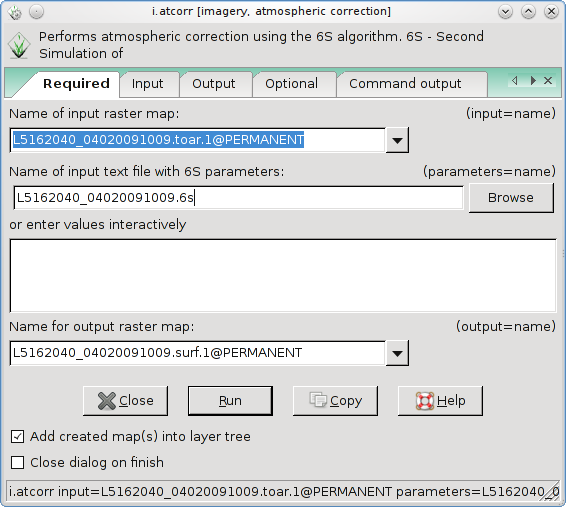
\includegraphics[scale=0.4]{gipe016.png}
   %caption of the figure
   \caption{i.atcorr Module}
   %label of the figure, which has to correspond to \ref{}:
   \label{fig:gipe016}
\end{figure}

For selection the DEM and visibility bands as input, while inside the i.atcorr go to input label and select the desired files. Visibility map has no more extra benefit when the value of visibility is written in parameter file. But DEM file can help to get better results of i.atcorr.\newline
Unlike the i.landsat.toar, the i.atcorr must be applied for every band individually for every given image.\newline


%\setkeys{Gin}{width=1\textwidth}
\begin{figure}[htbp]
   \centering
   %name of your graphic, without the path AND in PNG (screnshots etc)/PDF (drawings) format:
   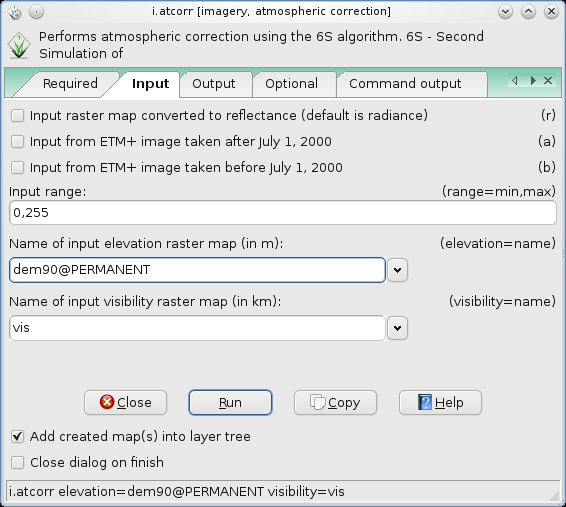
\includegraphics[scale=0.4]{gipe017.png}
   %caption of the figure
   \caption{i.atcorr Module Input Tab}
   %label of the figure, which has to correspond to \ref{}:
   \label{fig:gipe017}
\end{figure}


The script mentioned in \ref{appendixA}-4 can be used for automated approach of atmospheric correction for a set of  landsat images.\newline

The produced maps are reflectance at the surface for each band. The values range is between 0 and 1 showing the ratio of outgoing radiance to the incoming radiance at Earth Skin Surface.  
In order to test the reality of the generated values look to the NDVI values that can be produced by the red and near infrared band through map r.mapcalc module. The values related to green vegetation  area must be the highest. 

\section{Basic products creation}

Necessary images for energy balance calculation are NDVI, Albedo, Emissivity. These initial products have dedicated GRASS GIS modules.\newline

\subsection{NDVI production}
Vegetion index NDVI is a necessary basic product for some other higher level outputs such as Soil heat flux, Surface roughness (Z0m). It can be  calculated using "i.vi". Go to Imagery/Evapotranspiration calculation/vegetation indices, following the example below:\newline

%\setkeys{Gin}{width=1\textwidth}
\begin{figure}[htbp]
   \centering
   %name of your graphic, without the path AND in PNG (screnshots etc)/PDF (drawings) format:
   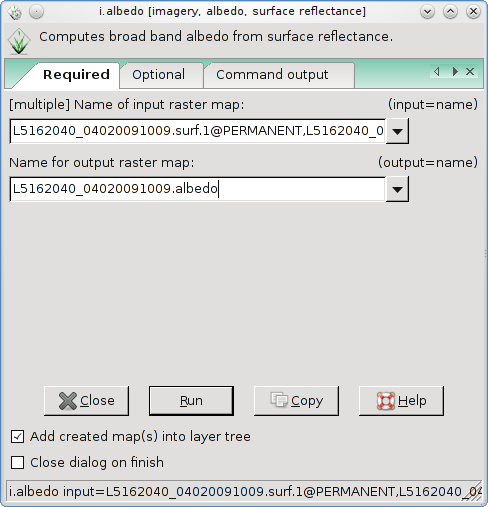
\includegraphics[scale=0.4]{gipe018.png}
   %caption of the figure
   \caption{i.vi Module}
   %label of the figure, which has to correspond to \ref{}:
   \label{fig:gipe018}
\end{figure}

There are 13 vegetation indices (VI) possibility in i.vi module. After selecting the desired name of red band, enter the name of VI (such as NDVI, EVI, DVI,...). Then go to Optional label and select the near infrared band for NDVI and the other bands is needed in case of the other VIs. \newline

%\setkeys{Gin}{width=1\textwidth}
\begin{figure}[htbp]
   \centering
   %name of your graphic, without the path AND in PNG (screnshots etc)/PDF (drawings) format:
   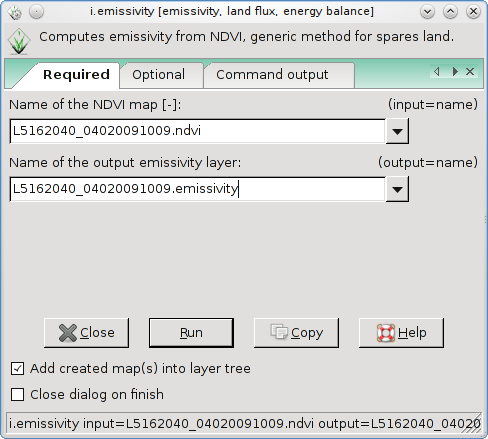
\includegraphics[scale=0.4]{gipe019.png}
   %caption of the figure
   \caption{i.vi Module}
   %label of the figure, which has to correspond to \ref{}:
   \label{fig:gipe019}
\end{figure}

\subsection{Albedo production}
Albedo is shortwave surface reflectance in range of 0.3 to 3.0 micro meters (figures are dimensionless).\newline 
Albedo is in fact an integration of the surface reflectance of all of the shortwave bands assuming a fraction for every band. The fractions for the bands are published by the landsat website and are as follow.
\begin{smallverbatim}
 Albedo = (0.293 * channel1 + 0.274 * channel2 \
        + 0.233 * channel3 + 0.156 * channel4 + \
        0.033 * channel5 + 0.011 * channel7)
\end{smallverbatim}
Albedo is calculated from the "i.albedo" module. It  computes broad band albedo from surface reflectance. This is an precursor to Soil heat flux, r.sun and Energy-Balance processing.\newline
Inside the GRASS windows, go to Imagery/Evapotranspiration calculation/Albedo, and select the the bands 1 to 5 and 7 of atmospherically corrected surface reflectance.\newline

%\setkeys{Gin}{width=1\textwidth}
\begin{figure}[htbp]
   \centering
   %name of your graphic, without the path AND in PNG (screnshots etc)/PDF (drawings) format:
   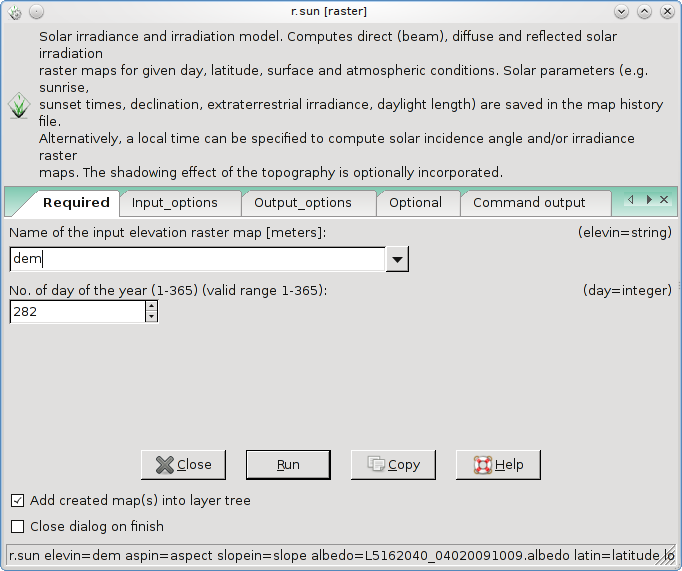
\includegraphics[scale=0.4]{gipe020.png}
   %caption of the figure
   \caption{i.albedo Module}
   %label of the figure, which has to correspond to \ref{}:
   \label{fig:gipe020}
\end{figure}

\subsection{Emissivity Production}
Surface emisivity is the ratio of the thermal energy radiated by the surface to the thermal energy  radiated by black body at the same temprature (is dimensionless).\newline 
The module i.emissivity calculates the emissivity in the longwave radiation spectrum, according to the semi-empirical equation related to NDVI by Caselles et al. (1997), valid in the NDVI range of 0.16 to 0.74. Estimation in the 8-14 micrometers range for sparse canopy.\newline

%\setkeys{Gin}{width=1\textwidth}
\begin{figure}[htbp]
   \centering
   %name of your graphic, without the path AND in PNG (screnshots etc)/PDF (drawings) format:
   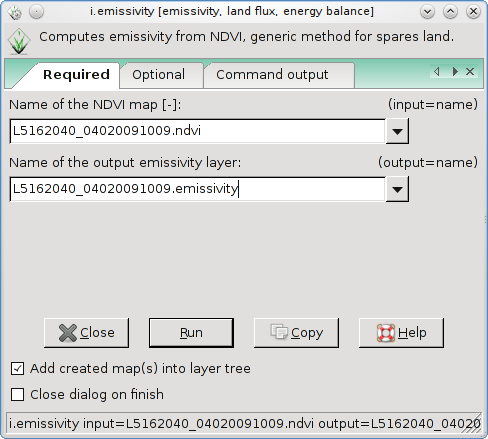
\includegraphics[scale=0.4]{gipe021.png}
   %caption of the figure
   \caption{i.emissivity Module}
   %label of the figure, which has to correspond to \ref{}:
   \label{fig:gipe021}
\end{figure}


\section{Energy balance terms}
The energy-balance models use visible, infrared and thermal remotely sensed data for solving the main equation:\newline
\begin{center}
Rn-G-H-$\lambda$ET=0 \newline
\end{center}
Where the Rn is the net radiation, H is the sensible heat flux, G is the soil heat flux, and $\lambda$ET is the latent heat flux.\newline
\subsection{Net Radiation}
Net radiation at satellite overpass (instantaneous) and integrated over the day are computed from a generic GRASS GIS raster module "r.sun". 
The r.sun program works in two modes. In the first mode it calculates for the image acquisition local time a solar incidence angle [degrees] and solar irradiance values [W.m-2]. In the second mode daily sums of solar radiation [Wh.m-2.day-1] are computed within a day.\newline

In the other hand, in mode 1, instantaneous net radiation, and in mode 2 the day integrated net radiation is computed. Both are necessary for the energy balance computation. Mode 1 for sensible heat flux computation and mode 2 for the Day ET potential.\newline

The model computes all three components of total radiation (beam, diffused and reflected) for the clear sky conditions, i.e. not taking into consideration the spatial and temporal variation of clouds. \newline

Note that the following raster inputs are recommended: aspect, slope, albedo, latitude and longitude. Slope and Aspect can be computed with "r.slope.aspect" using the DEM raster file, albedo with "i.albedo", latitude and longitude with "i.latlong".\newline

Run r.sun while inside the GRASS: go to Raster/Solar radiance and shadows/solar irradiance and irradiation. Input the name of DEM raster file and the Julian day of the year (image acquisition day). \newline

%\setkeys{Gin}{width=1\textwidth}
\begin{figure}[htbp]
   \centering
   %name of your graphic, without the path AND in PNG (screnshots etc)/PDF (drawings) format:
   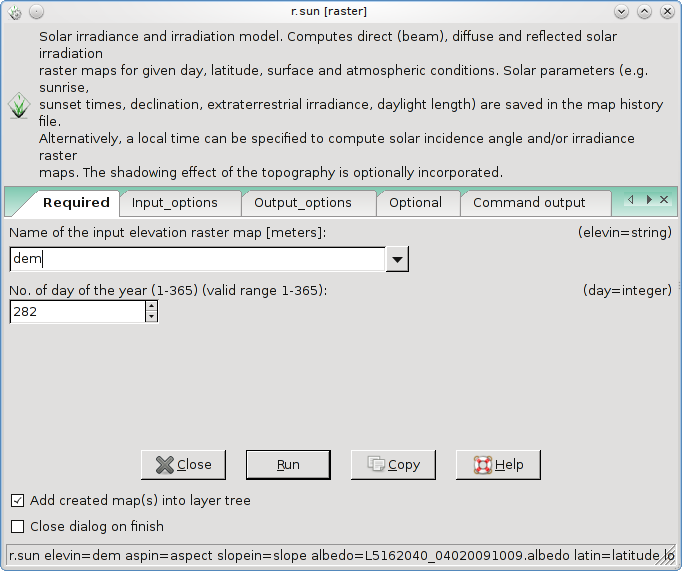
\includegraphics[scale=0.4]{gipe022.png}
   %caption of the figure
   \caption{r.sun Module}
   %label of the figure, which has to correspond to \ref{}:
   \label{fig:gipe022}
\end{figure}

To determine the other input file go to the input\_options label and input the slop, aspect, albedo, longitude and latitude files. The Linke atmospheric turbidity should be found in reference literature for the study area. The default is 3.0. Average monthly values of the Linke turbidity coefficient for a mild climate in the northern hemisphere is presented in \href{tab:001}.\newline

%\setkeys{Gin}{width=1\textwidth}
\begin{figure}[htbp]
   \centering
   %name of your graphic, without the path AND in PNG (screnshots etc)/PDF (drawings) format:
   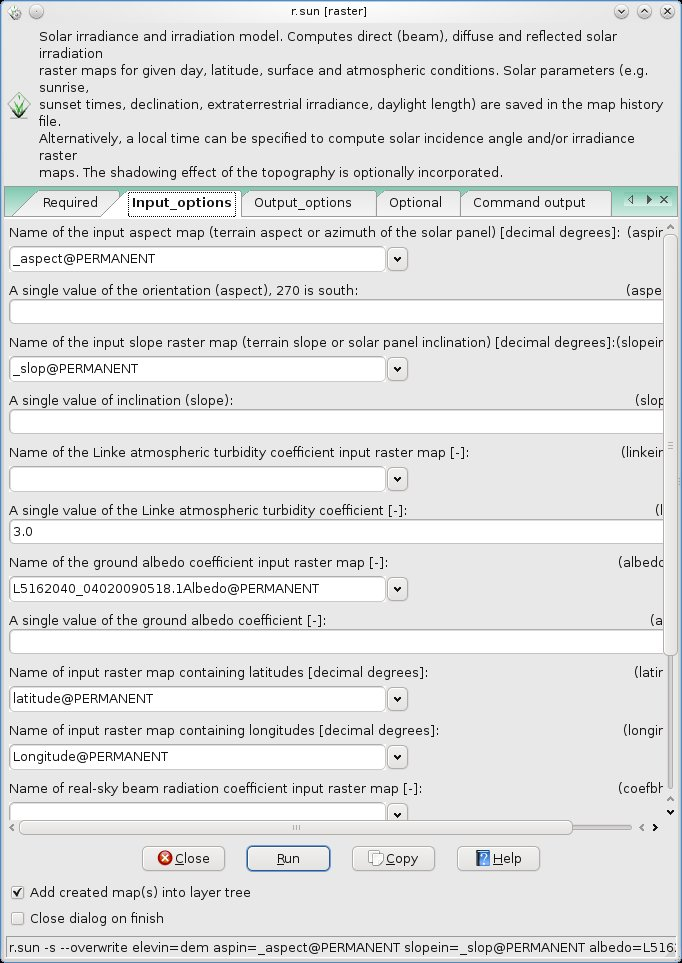
\includegraphics[scale=0.4]{gipe023.png}
   %caption of the figure
   \caption{r.sun Module, input options label}
   %label of the figure, which has to correspond to \ref{}:
   \label{fig:gipe023}
\end{figure}

Table 1: Linke Turbidity Coefficient
\begin{center}
\begin{tabular}{lllll}
Landscapes & Mountains & Rural & City & Industrial\\
January & 1.5 & 2.1 & 3.1 & 4.1\\
February & 1.6 & 2.2 & 3.2 & 4.3\\
March & 1.8 & 2.5 & 3.5 & 4.7\\
April & 1.9 & 2.9 & 4 & 5.3\\
May & 2 & 3.2 & 4.2 & 5.5\\
June & 2.3 & 3.4 & 4.3 & 5.7\\
July & 2.3 & 3.5 & 4.4 & 5.8\\
August & 2.3 & 3.3 & 4.3 & 5.7\\
September & 2.1 & 2.9 & 4 & 5.3\\
October & 1.8 & 2.6 & 3.6 & 4.9\\
November & 1.6 & 2.3 & 3.3 & 4.5\\
December & 1.5 & 2.2 & 3.1 & 4.2\\
Annual & 1.9 & 2.75 & 3.75 & 5
\end{tabular}
\linebreak
\end{center}

%\setkeys{Gin}{width=1\textwidth}
\begin{figure}[htbp]
   \centering
   %name of your graphic, without the path AND in PNG (screnshots etc)/PDF (drawings) format:
   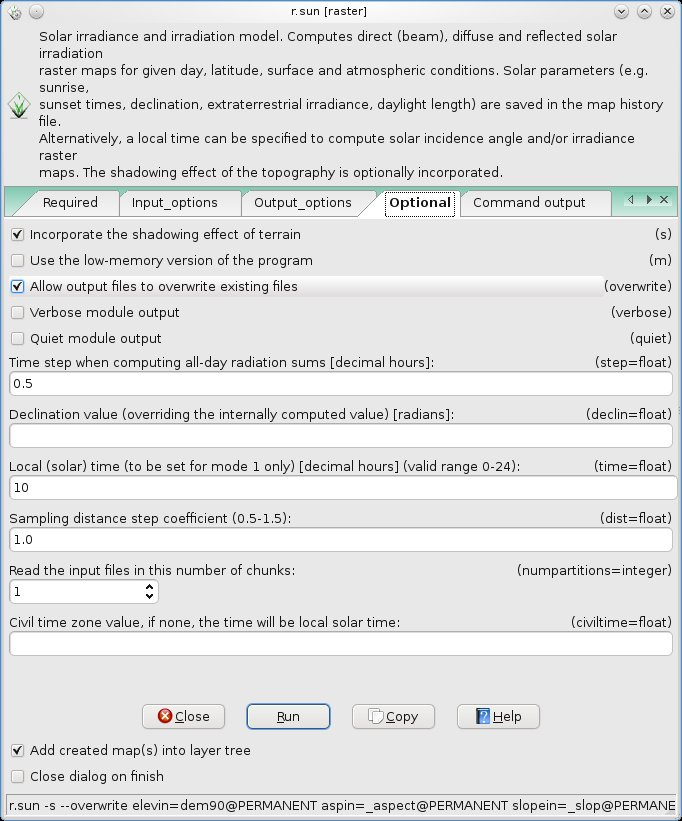
\includegraphics[scale=0.4]{gipe024.png}
   %caption of the figure
   \caption{r.sun Module, optional label}
   %label of the figure, which has to correspond to \ref{}:
   \label{fig:gipe024}
\end{figure}

In Optional label, push to the "Incorporate the shadowing effect of the terrain" and local (not GMT) time  of image acquisition.\newline
In Out\_option label write the name of desired output names. It is possible only to generate the output files for one of the Modes 1 and 2 in the same time.  So, add the desired names for 1,2,4,5 and 6 rows. Global or total irradiance output file is a product of the three base outputs Beam irradiance, Diffuse irradiance and reflected irradiance.\newline
To generate the output files for Mode 2, the r.sun must be run again and put all of the input files. In Output\_options the output files related to mode 2 or mod 1 and 2 must be filled (boxes 2 to 6) and the box 1 must be kept empty. In Optional label delete the local time which was mentioned for Mode 1 outputs in before.\newline

%\setkeys{Gin}{width=1\textwidth}
\begin{figure}[htbp]
   \centering
   %name of your graphic, without the path AND in PNG (screnshots etc)/PDF (drawings) format:
   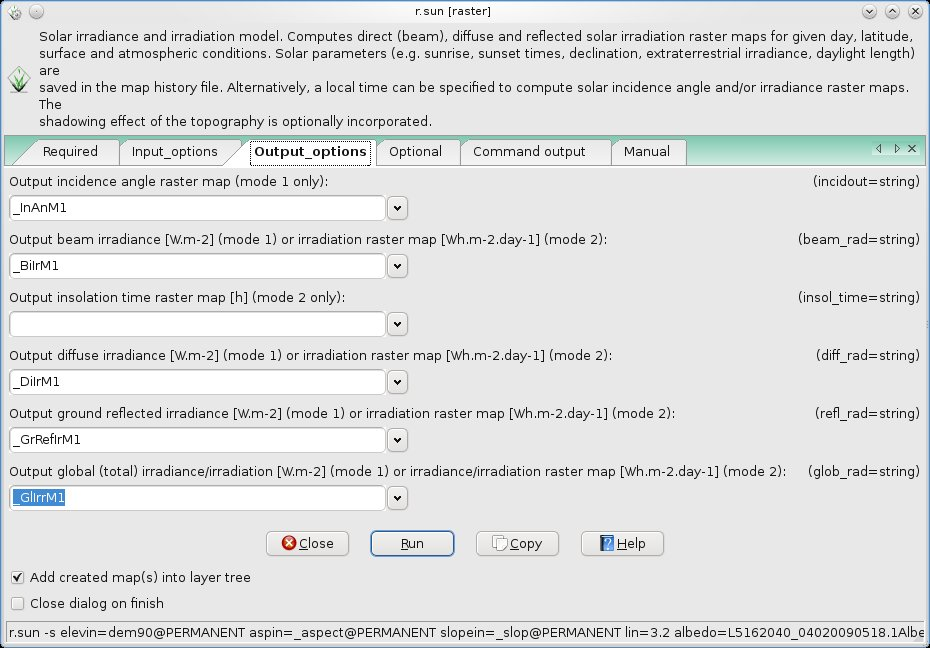
\includegraphics[scale=0.3]{gipe025.png}
   %caption of the figure
   \caption{r.sun Mode 1}
   %label of the figure, which has to correspond to \ref{}:
   \label{fig:gipe025}
\end{figure}

%\setkeys{Gin}{width=1\textwidth}
\begin{figure}[htbp]
   \centering
   %name of your graphic, without the path AND in PNG (screnshots etc)/PDF (drawings) format:
   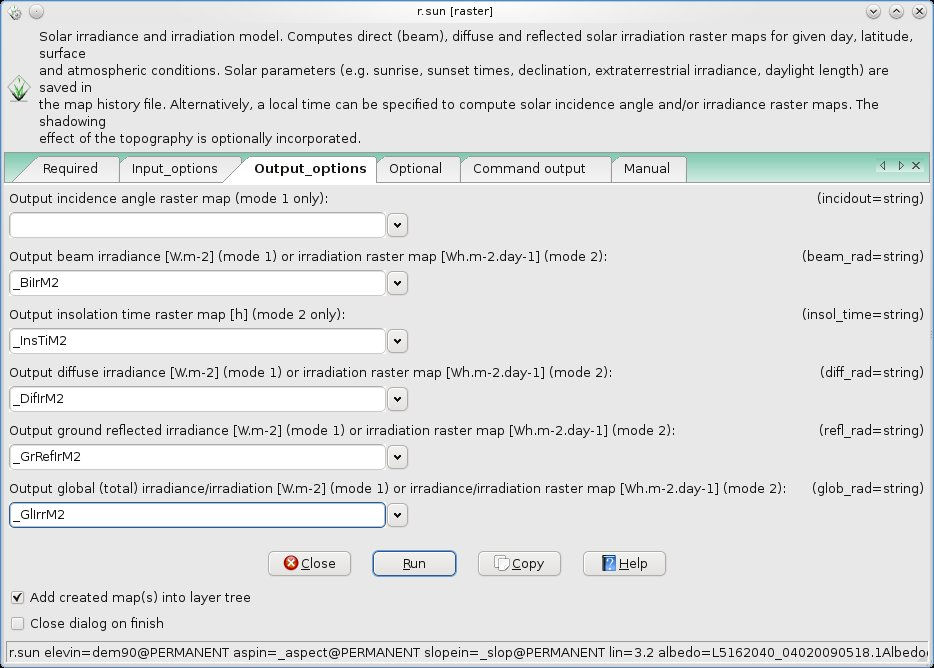
\includegraphics[scale=0.3]{gipe025a.png}
   %caption of the figure
   \caption{r.sun Mode 2}
   %label of the figure, which has to correspond to \ref{}:
   \label{fig:gipe025a}
\end{figure}

Incident angle raster map is computed using DEM, aspect, slope maps for the given julian day and local time. The figures ranges between 0 and 90.\newline
Global or total irradiance output file is a product of the three basal outputs beam irradiance, diffuse irradiance and reflected irradiance. \newline
The range of values of the products is dependent of many factors but some guidelines can be given as followings:\newline\linebreak
The range of figures for Beam irradiance are normaly between 500 to 1000, diffuse irradiance between 70 to 150, and ground reflected irradiance between less than 1 to 100 all in (W/m2).\newline
The summation of those basal products figures (global irradiance) for a given pixel must be less than actual instantaneous radiation at the atmosphere which ranged between 1361 to 1386 (W/M2).\newline\linebreak
The net radiation (W/M2/day) value for each pixel can be computed by dividing the global irradiation mode 2 (Wh/M2/day) by the actual sunshine hours. It may be called Rnet.day product.\newline
Sunshine hours is a weather station parameter and alternatively is possible to generate as a raster file by using the i.sunhours module.\newline\linebreak
The r.sun command line for mode 1 and mode 2 are as followings and can be used for automated scripting.\newline\linebreak

Mode 1
\begin{smallverbatim}
 r.sun elevin=dem90
  aspin=_aspect slopein=_slop lin=3.2
  albedo=L5162040_04020090518.1Albedo
  latin=latitude longin=Longitude
  incidout=_InAnM1 beam_rad=_BiIrM1
  diff_rad=_DifIrM1 refl_rad=_GrRefIrM1
  glob_rad=_GlIrrM1 day=138 time=10
\end{smallverbatim}

Mode 2
\begin{smallverbatim}
 r.sun elevin=dem90
  aspin=_aspect slopein=_slop lin=3.2
  albedo=L5162040_04020090518.1Albedo
  latin=latitude longin=Longitude
  beam_rad=_BiIrM2 insol_time=_InsTiM2
  diff_rad=_DifIrM2 refl_rad=_GrRefIrM2
  glob_rad=_GlIrrM2 day=138
\end{smallverbatim}


\subsection{soil heat flux}
The generic module "i.eb.soilheatflux" calculates the soil heat flux approximation (g0). It takes input of Albedo, NDVI, Surface Skin temperature, Net Radiation (see r.sun), and time of satellite overpass.\newline
Surface temperature (LST) is directly relative to thermal radiation recorded in thermal band . So the the thermal band that has been converted to radiation (by i.landsat.toar) can be used as the input file for surface temperature raster map.\newline 
Net radiation is the global radiation product of mode1 of r.sun module.\newline
Time raster map can be created by map calculation knowing the local time of satellite overpass.\newline

Soil heat flux can be computed with "i.eb.g0".\newline

%\setkeys{Gin}{width=1\textwidth}
\begin{figure}[htbp]
   \centering
   %name of your graphic, without the path AND in PNG (screnshots etc)/PDF (drawings) format:
   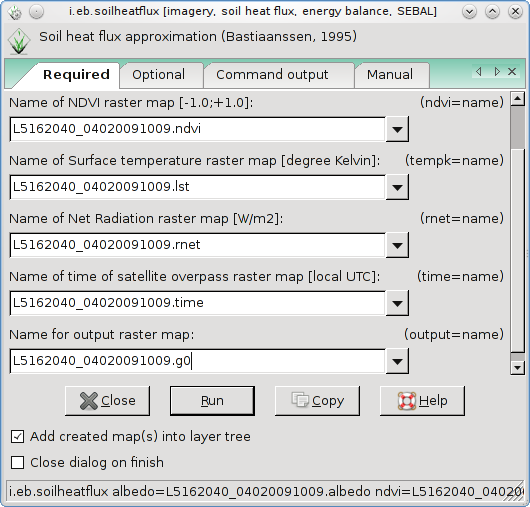
\includegraphics[scale=0.4]{gipe026.png}
   %caption of the figure
   \caption{i.eb.soilheatflux Module}
   %label of the figure, which has to correspond to \ref{}:
   \label{fig:gipe026}
\end{figure}

The i.eb.soilheatflux command line is as followings and can be used for automated scripting.
\begin{smallverbatim}
i.eb.soilheatflux \
    albedo="L5162040_04020090518.1Albedo" \
    ndvi="L5162040_04020090518.1NDVI" \
    tempk="L5162040_04020090518.toar.6" \
    rnet="_GlIrrM1" time="time" output="_G0" 
\end{smallverbatim}

\subsection{Sensible Heat Flux}
The Sensible heat flux (H) is calculated by "i.eb.h\_SEBAL01", given both maps of Net Radiation and soil Heat flux (Rn, G) at instantaneous time, the surface roughness (z0m), a map of the altitude corrected temperature (t0dem), a point data of the frictional velocity (u*), a value of actual vapour pressure (ea[KPa]) and the (x,y) pairs for wet and dry pixels.\newline
Surface roughness (Z0m) is an dependent variable of vegetation height. Generation of an accurate map of the vegetation inside the study area in the date of image acquisition will lead to increase the accuracy of H calculation.\newline
\begin{smallverbatim}
    Z0m=hveg * 0.136 
\end{smallverbatim}
hveg is the height of vegetation (m).\newline
Altitude corrected temperature map can be computed by using the toar thermal band and the DEM.\newline
\begin{smallverbatim}
    T0DEM=LST-(0.00627*DEM)
\end{smallverbatim}
The factor 0.00627 is the gradient of decreasing the temprature in relation to the increase in height (6.27 degree in each 1000 meter).\newline

The U* (Called U star) is the friction velocity is computed by:\newline
\begin{smallverbatim}
    U*= 0.41*um/(ln(hu/Z0m) 
\end{smallverbatim}
um is wind speed in the time of satellite overpass (m/s), hu is the height of wind measurement which is normally described as 5 (m). Z0m here is not the same as that is used in  U* calculation. The  hveg in this case is defined as the height of vegetation around the weather station.\newline

The value of actuale vapor pressure ea is calculated using the e0 for max and min tempreture.\newline
\begin{smallverbatim}
    e0=0.618*exp(17.27*T/(T+273.3))  
\end{smallverbatim}
e0 is the saturation vapor pressure at the air temperature. It must be calculated for Max and Min absolute tempreture.\newline
ea is calculated using:\newline
\begin{smallverbatim}
    ea=RH*(e0Max+e0Min)/2))/100  
\end{smallverbatim}
RH is the measured relative humidity at the time of satellite overpass.\newline
The location (row and column) of the wet (cold) and dry (hot) pixel must be found by the user. For wet pixel a place inside a water body and for dry pixel a place inside a bare and dry soil surface is recommended (SEBAL method is geographically dependent on extrem energy balance points).\newline

%\setkeys{Gin}{width=1\textwidth}
\begin{figure}[htbp]
   \centering
   %name of your graphic, without the path AND in PNG (screnshots etc)/PDF (drawings) format:
   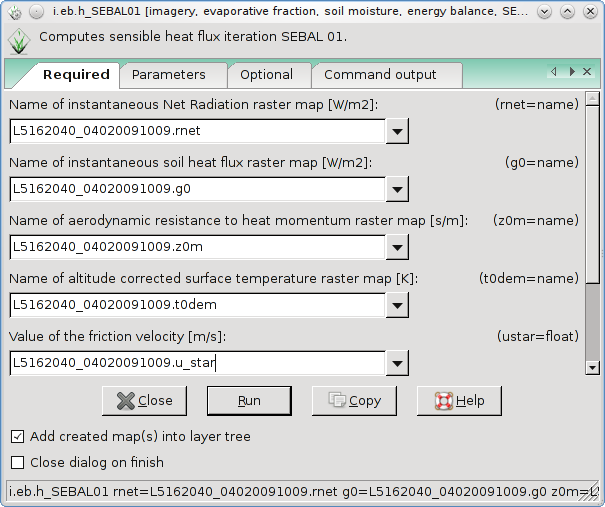
\includegraphics[scale=0.4]{gipe027.png}
   %caption of the figure
   \caption{i.eb.h\_SEBAL01 Module}
   %label of the figure, which has to correspond to \ref{}:
   \label{fig:gipe027}
\end{figure}

Note that additional images should be created about surface roughness length (z0m), altitude corrected temperature (t0dem), the height independent wind speed (U*), along with coordinates of the "wet" and "dry" pixels (SEBAL method is geographically dependent on extrema energy balance points). \newline

\subsection{Evaporative Fraction}
Evaporative fraction can be calculated by "i.eb.evapfr":\newline

%\setkeys{Gin}{width=1\textwidth}
\begin{figure}[htbp]
   \centering
   %name of your graphic, without the path AND in PNG (screnshots etc)/PDF (drawings) format:
   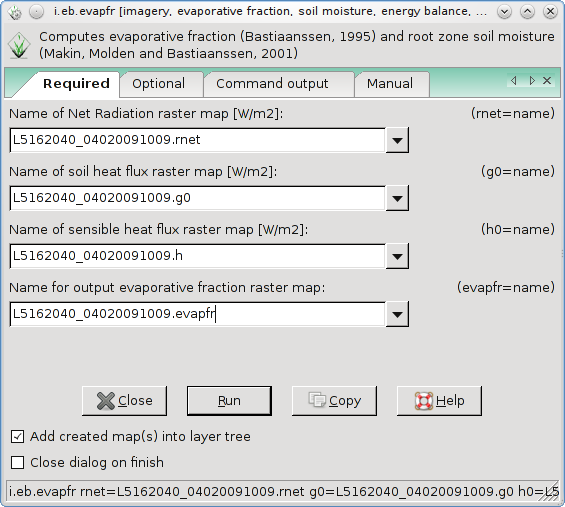
\includegraphics[scale=0.4]{gipe028.png}
   %caption of the figure
   \caption{i.eb.evapfr Module}
   %label of the figure, which has to correspond to \ref{}:
   \label{fig:gipe028}
\end{figure}

\subsection{Evapotranspiration}
Evapotranspiration can be computed from "i.eb.eta":\newline

%\setkeys{Gin}{width=1\textwidth}
\begin{figure}[htbp]
   \centering
   %name of your graphic, without the path AND in PNG (screnshots etc)/PDF (drawings) format:
   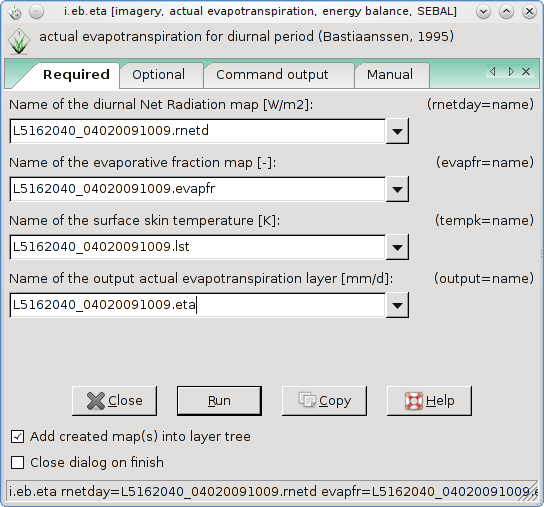
\includegraphics[scale=0.4]{gipe029.png}
   %caption of the figure
   \caption{i.eb.eta Module}
   %label of the figure, which has to correspond to \ref{}:
   \label{fig:gipe029}
\end{figure}

\newpage


\section{Appendix A: GRASS SCRIPTS}
\label{appendixA}

\subsection{Unzipping the tarball compressed files}

For Linux users in Terminal and for Windows users in Dos prompt window should be written:\newline

\begin{smallverbatim}
for file in *.tar.gz
do
tar -xvzf \$file
done
\end{smallverbatim}

Control should be given to run the script in the same directory as the images are in.\newline

\subsection{Renaming and importing}
In GRASS Command Line Interface (CLI) write the script:

\begin{smallverbatim}
echo "RUN from the MTL.txt directory and \
 within the GRASS environment"

for file in L5*0.TIF
do
	out=\$(echo \$file | sed 's/\\(.*\) 
        \_\\(.*\)\_B\\(.*\)0.TIF/\1\\_\2\.\3/g')
	echo \$out
	r.in.gdal input=\$file output=\$out
done
\end{smallverbatim}

For more information about this script, refer to "sed" program manual in Unix/Linux and to the "r.in.gdal" help in GRASS GIS.
 
\subsection{Conversion of DN to radiance}
Conversion of DN to reflectance at top of atmosphere (TOAR) is done with the script:

\begin{smallverbatim}
echo "RUN from the MTL.txt directory and within \
 the GRASS environment"

path=162
row=040

for L5_MTL_file in L5\$path\$row*_MTL.txt
do
	L5_prefix=\$(echo \$L5_MTL_file \| \
	  sed 's/\\(.*\)_MTL.txt/\\1/')

	i.landsat.toar -t \
	  input_prefix=\$L5_prefix\. \
	  output_prefix=\$L5_prefix.toar.  \
	  metfile=/home/user1/\$L5\_MTL\_file \
	  sensor=tm5
done
\end{smallverbatim}


This script requires to change the path and row of the target images you are processing.\newline

\subsection{Atmospheric correction with i.atcorr}
Script for atmospheric correction by 6S method for landsat 5 TM.\newline

\begin{smallverbatim}
#!/bin/bash
# Basic script for i.atcorr for L 5 TM

#Geometrical conditions (L5TM)
geom=7
#Sensor height (satellite is -1000)
sens_height=-1000

#Here we suppose you have altitude (DEM) and \
 Visibility (VIS) maps ready
#--------------------------------------------- 
#Visibility dummy value (overwritten by VIS \
 raster input)
vis=9
r.mapcalc expression="visibility=\$vis" \
 --overwrite

#Altitude dummy value (in Km should be negative\
 in this param file)
#(overwritten by DEM raster input)
alt=-1.200

#---------------------------
# Please change as you need
#---------------------------
# L5 basename as stored in GRASS GIS and used \
 by i.landsat.toar
L5basename=L5162040\_04020090705

# Location of parameter file
root=/home/icwater/

#datetime of satellite overpass (month, day, \
 GMT decimal hour)
mdh="7 5 6.30"

# Central Lat/Long
Long=51.410
Lat=24.234

#Atmospheric mode
atm\_mode=6 #us standard 62 (for lack of more\
 precise model)

#Aerosol model
aerosol\_mode=1 #continental

#satellite band number (L5TM [25,26,27,28,29,30])
satbandno=25 #Band 1 of L5TM is first to undergo\
 atmospheric correction

for bandno in 1 2 3 4 5 7
do # Generate the parameterization file
	echo "\$geom                            \
         - geometrical conditions=Landsat 5 TM" \
         > \$root/param\_L5.txt
	echo "\$mdh \$Long \$Lat   \
         - month day hh.ddd longitude latitude \
         ("hh.ddd" is in decimal hours GMT)" >>\
         \$root/param\_L5.txt
	echo "\$atm\_mode                       \
         - atmospheric mode=tropical" >> \
         \$root/param\_L5.txt
	echo "\$aerosol\_mode                   \
         - aerosols model=continental" >>\
         \$root/param\_L5.txt
	echo "\$vis                           \
         - visibility [km] (aerosol model \
         concentration), not used as there is \
         raster input" >> \$root/param\_L5.txt
	echo "\$alt                       \
         - mean target elevation above sea level\
         [km] (here 600m asl), not used as there \
         is raster input" >> \$root/param\_L5.txt
	echo "\$sens\_height                     \
         - sensor height (here, sensor on board a\
         satellite)" >> \$root/param\_L5.txt
	echo "\$satbandno                        \
         - 'i'th band of TM Landsat 5" >>\
         \$root/param\_L5.txt
	# Process band-wise atmospheric correction with 6s
	i.atcorr -r -o -f \
         input=\$L5basename.toar.\$bandno\
         elevation=dem90 visibility=vis \
         parameters=\$root/param\_L5.txt \
         output=\$L5basename.surf.\$bandno \
         range=0,1 rescale=0,1 --overwrite
	# Increment satellite band number 
	satbandno=\$((satbandno+1))
done  
\end{smallverbatim}


\address{GRASS Development Team\\
  \url{http://grass.osgeo.org}\\
  \email{tmitchell@osgeo.org}}

%%% Local Variables: 
%%% mode: latex
%%% TeX-master: main\_document.tex
%%% End: 

